\subsection{DIAGRAMM}
\begin{figure}[H]
  \centering
  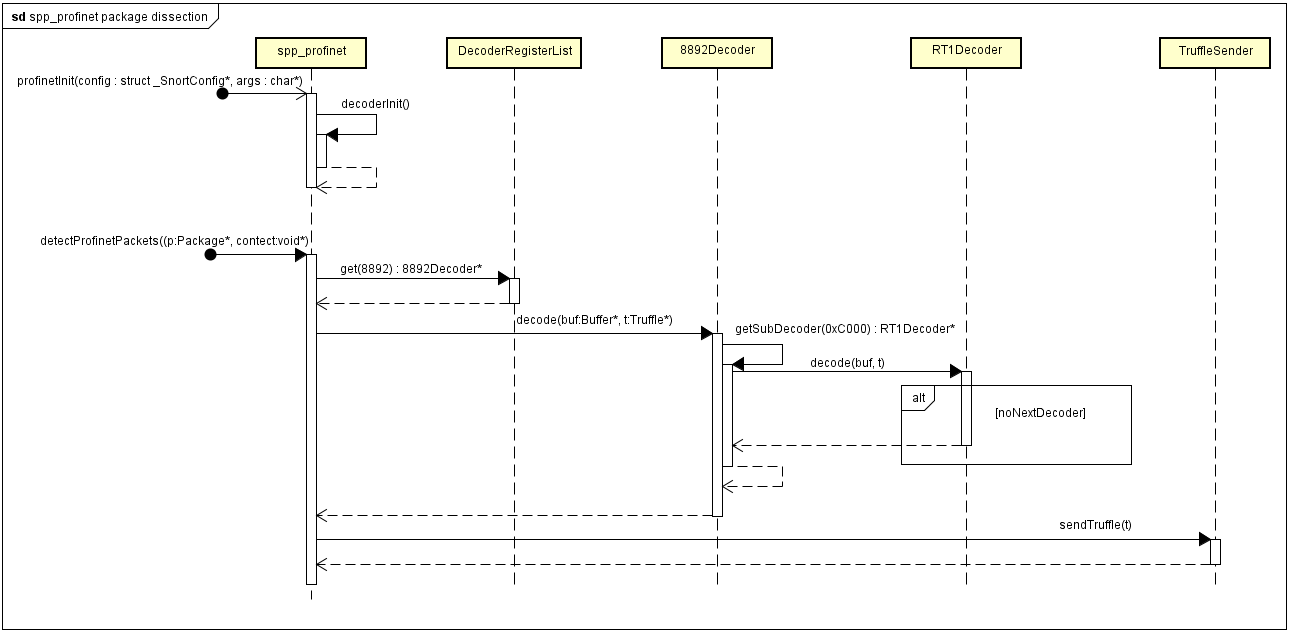
\includegraphics[width=\textwidth]{../diagramimages/spp-profinet-package-dissection.png}
  \caption[Sequenzdiagramm DIAGRAMM]{Sequenzdiagramm DIAGRAMM}
\end{figure}

In diesem Diagramm wird die Ausführung des LoadSnapshotCommand dargestellt. Der Command wird von der View erstellt, falls der Benutzer versucht Replays anzusehen. Der Command ruft load() in dem ReplayLogLoadService auf. Dieser nimmt das übergebene Instant an und deserialisiert damit den ReplayLog. Dieser liefert den Graphen und die Commands. Im Proxy, der für den Replaygraph zuständig ist, wird der geladene Graph referenziert. Danach wird im ReplayLogLoadService das play-Flag gesetzt (da Service im eigenen Thread läuft, was zwecks besserer Übersicht ausgelassen wurde) und im NetworkGraphSwitch wird der aktuell dargestellte Graphen auf den Replaygraph umgestellt.